\documentclass[../hw.tex]{subfiles}

\begin{document}

\begin{center}
    \section*{Homework 1}
    \addcontentsline{toc}{section}{Homework 1}
    \subsection*{Due 1/24 9pm}
\end{center}
\hrule \vspace{10px}
\paragraph{1.} Given: the 2D Cartesian relation to polar coordinates
\begin{align*} \tag{1} \label{eq:1}
    \vu{r} = \vu{x} \cos \phi + \vu{y} \sin \phi, \quad
    \vu{\phi} = -\vu{x} \sin \phi + \vu{y} \cos \phi
\end{align*}
% figure of fig1.png
% \begin{figure}[ht]
%     \centering
%     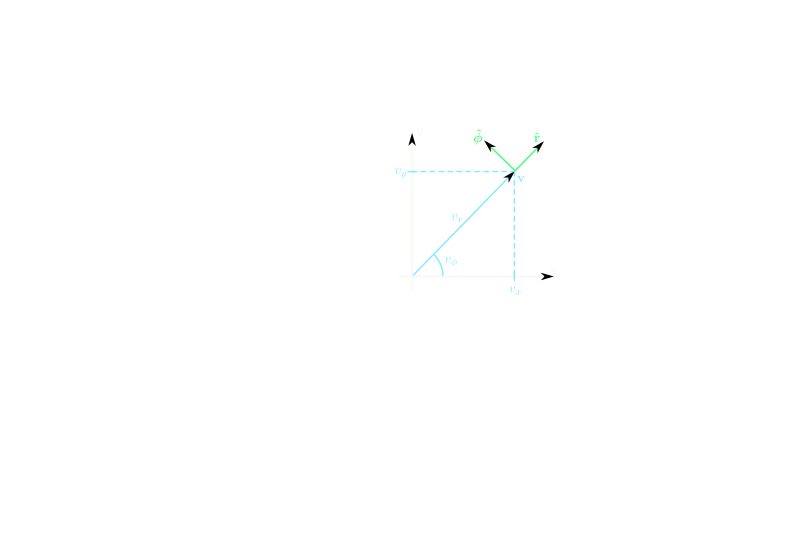
\includegraphics[width=0.4\linewidth]{fig1.png}
%     \caption{2D Cartesian to Polar Coordinates. Using simple Geometry, we can create a right
%     triangle with sides $v_x, v_y, v_r$.}
%     \label{fig:1.1}
% \end{figure}

% From Figure \ref{fig:1.1} the Cartesian vector components are
% \begin{align*}
%     v_x = v_r \cos v_\phi, \quad v_y = v_r \sin v_\phi
% \end{align*}
% The Pythagorean theorem gives the radial component
% \begin{align*}
%     v_r = \sqrt{v_x^2 + v_y^2}
% \end{align*}
% and the angular component is simply
% \begin{align*}
%     v_\phi = \arctan(\frac{v_y}{v_x})
% \end{align*}
We can write $v$ as a linear combination of $\vu{r}$ and $\vu{\phi}$
\begin{align*}
    \vb{v} &= v_r \vu{r} + v_\phi \vu*{\phi} \\
    &= v_r (\vu{x} \cos \phi + \vu{y} \sin \phi) + v_\phi (-\vu{x} \sin \phi + \vu{y} \cos \phi) \\
    &= (v_r \cos \phi - v_\phi \sin \phi) \vu{x} + (v_r \sin \phi + v_\phi \cos \phi) \vu{y}
\end{align*}
and since we know the vector in Cartesian coordinates is
\begin{align*}
    \vb{v} = v_x \vu{x} + v_y \vu{y}
\end{align*}
we can equate the components to get
\begin{align*}
    v_x &= v_r \cos \phi - v_\phi \sin \phi \\
    v_y &= v_r \sin \phi + v_\phi \cos \phi
\end{align*}
multiplying the first equation by $\cos\phi$ and the second by $\sin\phi$ and adding them together
\begin{align*}
    v_x \cos\phi &= v_r \cos^2\phi - v_\phi \sin\phi\cos\phi \\
    v_y \sin\phi &= v_r \sin^2\phi + v_\phi \sin\phi\cos\phi \\
    v_x \cos\phi + v_y \sin\phi &= v_r (\cos^2\phi + \sin^2\phi)
\end{align*}
or simply
\begin{align*}
    v_r = v_x \cos\phi + v_y \sin\phi
\end{align*}
Likewise,
\begin{align*}
    v_y \cos\phi &= v_r \sin\phi\cos\phi + v_\phi \sin^2\phi \\
    v_x \sin\phi &= v_r \sin\phi\cos\phi - v_\phi \cos^2\phi
\end{align*}
and subtracting the second equation from the first
\begin{align*}
    v_y \cos\phi - v_x \sin\phi &= v_\phi (\sin^2\phi + \cos^2\phi)
\end{align*}
Therefore we get the components of $\vb{v}$ in polar coordinates
\begin{align*}
    &\boxed{v_r = v_x \cos\phi + v_y \sin\phi} \\
    &\boxed{v_\phi = - v_x \sin\phi + v_y \cos\phi}
\end{align*}
Since $\vu{x}$ and $\vu{y}$ are \emph{constant}, the time derivatives of \eqref{eq:1} are
\begin{align*}
    \dot{\vu{r}} = \dv{t} \vu{r} &= \vu{x} \dv{t}(\cos\phi) + \vu{y} \dv{t}(\sin\phi) \\
    &= (-\dot\phi \sin\phi) \vu{x} + (\dot\phi \cos\phi) \vu{y} = \dot\phi \vu{\phi}
\end{align*}
and
\begin{align*}
    \dot{\vu{\phi}} = \dv{t} \vu{\phi} &= -\vu{x} \dv{t}(\sin\phi) + \vu{y} \dv{t}(\cos\phi) \\
    &= (-\dot\phi \cos\phi) \vu{x} + (-\dot\phi \sin\phi) \vu{y} = -\dot\phi \vu{r}
\end{align*}

\paragraph{2.}
From Taylor Problem 1.45: [\emph{Hint:} Consider the derivative of $ \vb{v}^2$].

Since the magnitude of $\vb{v}(t)$ is also $\sqrt{\vb{v}(t) \cdot \vb{v}(t)}$, the derivative of 
$\vb{v}^2$ is tells us if the magnitude is constant.
\begin{align*}
    \dv{t} \vb{v}^2 &= \dv{t} (\vb{v}(t) \cdot \vb{v}(t)) \\
    &= 2 \dot{\vb{v}}(t) \cdot \vb{v}(t)
\end{align*}

The magnitude of $\vb{v}(t)$ is constant if $\dv{t} \vb{v}^2 = 0$. Since the dot product is zero, 
$\vb{v}(t)$ is orthogonal to $\dot{\vb{v}}(t)$.

\paragraph{3.}
Using the product rule for the dot product $\dv{t}(\vb{x} \vdot \vb{y}) = \dot{\vb{x}} \vdot \vb{y}
+ \vb{x} \vdot \dot{\vb{y}}$
\begin{align*}
    \frac{d}{dt} [\vect{a} \cdot (\vect{v} \times \vect{r})] 
    &= \frac{d\vect{a}}{dt} \cdot (\vect{v} \times \vect{r}) 
    + \vect{a} \cdot \frac{d}{dt} (\vect{v} \times \vect{r}) \\
    &= \vect{\dot a} \cdot (\vect{v} \times \vect{r}) 
    + \vect{a} \cdot \frac{d\vect{v}}{dt} \times \vect{r} 
    + \vect{a} \cdot \vect{v} \times \frac{d\vect{r}}{dt} \\
    &= \vect{\dot a} \cdot (\vect{v} \times \vect{r}) 
    + \vect{a} \cdot \vect{a} \times \vect{r} + \vect{a} \cdot \vect{v} \times \vect{v} \\
    &= \vect{\dot a} \cdot (\vect{v} \times \vect{r})
\end{align*}

The cross product of a vector with itself is zero ($\vect{v} \times \vect{v} = 0$), and the dot 
product of orthogonal vectors are zero (acceleration and position are perpendicular based on the
result from Problem 2) QED

\paragraph{4.} Given
\begin{align*} \tag{3}
    \ddot \theta = -\frac{g}{l} \sin \theta
\end{align*}
(a) Moving everything to one side:
\begin{align*}
    \ddot \theta + \frac{g}{l} \sin \theta = 0
\end{align*}
multiplying by $\dot\theta$ and grouping terms:
\begin{align*}
    \dot\theta \ddot \theta + \frac{g}{l} \dot\theta \sin \theta &= 0 \\
    \dot\theta \dv{t}(\dot\theta) + \frac{g}{l} \sin\theta \dv{t}(\theta) &= 0 \\
    \dv{t}(\frac{1}{2} \dot\theta^2) - \dv{t}(\frac{g}{l} \cos\theta) &= 0 \\
    \dv{t}(\frac{1}{2} \dot\theta^2 - \frac{g}{l} \cos\theta) &= 0
\end{align*}
so the integral constant is
\begin{align*}
    \frac{1}{2} \dot\theta^2 - \frac{g}{l} \cos\theta = C
\end{align*}
Initially the pendulum starts at rest, $\dot\theta(t=0) = 0$ and $\theta(0) = \theta_o$ thus
\begin{align*}
    \boxed{C = -\frac{g}{l} \cos\theta_o}
\end{align*}

(b) Rewriting $X=C$
\begin{align*}
    \frac{1}{2} \dot\theta^2 - \frac{g}{l} \cos\theta &= -\frac{g}{l} \cos\theta_o \\
    \dot\theta &= \sqrt{\frac{2g}{l} (\cos\theta - \cos\theta_o)}
\end{align*}
using separation of variables
\begin{align*}
    \dd{\theta} = \sqrt{\frac{2g}{l} (\cos\theta - \cos\theta_o)} \dd{t}
\end{align*}
Integrating gives the analytic solution
\begin{align*}
    \boxed{\theta(t) = \sqrt{\frac{2g}{l}} \int_0^T \sqrt{\cos\theta - \cos\theta_o} \dd{t}}
\end{align*}
where $T$ is the period of the pendulum.

(c) The period of the pendulum is the time it takes to complete one cycle. Since
\begin{align*}
    \dot\theta = \dv{\theta}{t}
\end{align*}
using separation of variables
\begin{align*}
    \dd{t} = \frac{1}{\dot\theta} \dd{\theta}
\end{align*}
Integrating both sides gives the period
\begin{align*}
    \int &\dd{t} = \int \frac{1}{\dot\theta} \dd{\theta} \\
    &\boxed{T = 4\sqrt{\frac{l}{2g}}
    \int_0^{\theta_o} \frac{1}{\sqrt{\cos\theta - \cos\theta_o}} \dd{\theta}}
\end{align*}
where the constant `4' comes from the fact that the total cycle is 4 times the period it takes to go
from path from $\theta_o$
to $0$.
\end{document}